\documentclass[12pt, a4paper]{article}
\usepackage{graphicx}
\usepackage{xcolor}
\usepackage{pgfplots}
\usepackage[german]{babel}
\pgfplotsset{width=\textwidth,height=8cm,compat=1.9}
\renewcommand{\contentsname}{Inhaltsverzeichnis}
\renewcommand{\figurename}{Abb.}
\newcommand\crule[3][black]{\textcolor{#1}{\rule{#2}{#3}}}

\begin{document}
\begin{titlepage}
\begin{center}
    \large{Protokoll} \\
    \LARGE{Bestimmung der Wellenlängen der Spektrallinien einer Wasserstofflampe} \\
    \Large{Balmer-Serie} \\
    \vspace{10mm}
    \small{Ort} \\
    \Large{ BBS Papenburg,\\ 
            Raum B007a} \\
    \vspace{10mm}
    \small{Zeitraum} \\
    \Large{ 14.01.2021 \\
            13:45 - 15:15} \\
    \vspace{15mm}
    \small{Protokollanten} \\
    \Large{ Mathis Mensing, \\
            Felix Schmees }
\end{center}

\thispagestyle{empty}
\end{titlepage}

\tableofcontents
\newpage

\section{Ziel des Experiments}
Das Ziel des Experiments ist es, die Wellenlängen der Emissionsspektrallinien einer Wasserstofflampe zu bestimmen.

\subsection{Theorie}
$\Delta s = k * \lambda$ \\
1: $\sin a = \frac{\Delta s}{g} = \frac{k * \lambda}{g}$ \\
2: $\tan a = \frac{x}{l}$ \\
3: $\Rightarrow a = \arctan \frac{x}{l}$ \\\\
3 in 1:\\
$\sin(\arctan(\frac{x}{l})) = \frac{\lambda}{g}$ \\
$\lambda = \sin(\arctan(\frac{x}{l})) * g$

\section{Versuchsaufbau}
\subsection{Materialien}

\begin{itemize}
    \item Wasserstofflampe
    \item Hochspannungsnetzteil
    \item Spalt
    \item Diffraktionsgitter (600 Striche/mm)
    \item Maßstab
    \item Geradlinige Schiene (mit Maßlinien)
    \item 3 Stativhalterungen (Schlitten)
\end{itemize}

\newpage

\subsection{Aufbau}
Die geradlinige Schiene wird orthogonal zu einem Schirm (in diesem Fall einer weißen Wand) aufgestellt.
Der Maßstab wird direkt parallel am Schirm angebracht.
Die Wasserstofflampe wird in einer Stativhalterung befestigt und am Schirmende der Schiene platziert.
Der Spalt wird direkt vor der Wasserstofflampe montiert, sodass dieser in einer Linie parallel zur Schiene zur Lampe steht.
Das Diffraktionsgitter wird nun in einem gewissen Abstand vom Schirm platziert, sodass eine virtuelle Abbildung der Spektrallinien durch dieses möglich ist.
Dieser Abstand wird im Verlauf des Experiments angepasst.
Zuletzt wird die Wasserstofflampe an das Hochspannungsnetzteil angeschlossen und eingeschaltet.

Es ist wichtig, dass alle Elemente auf der Schiene in einer geraden Linie stehen, sodass das Licht nicht blockiert wird.

\begin{figure}[p]
    \centering
    
    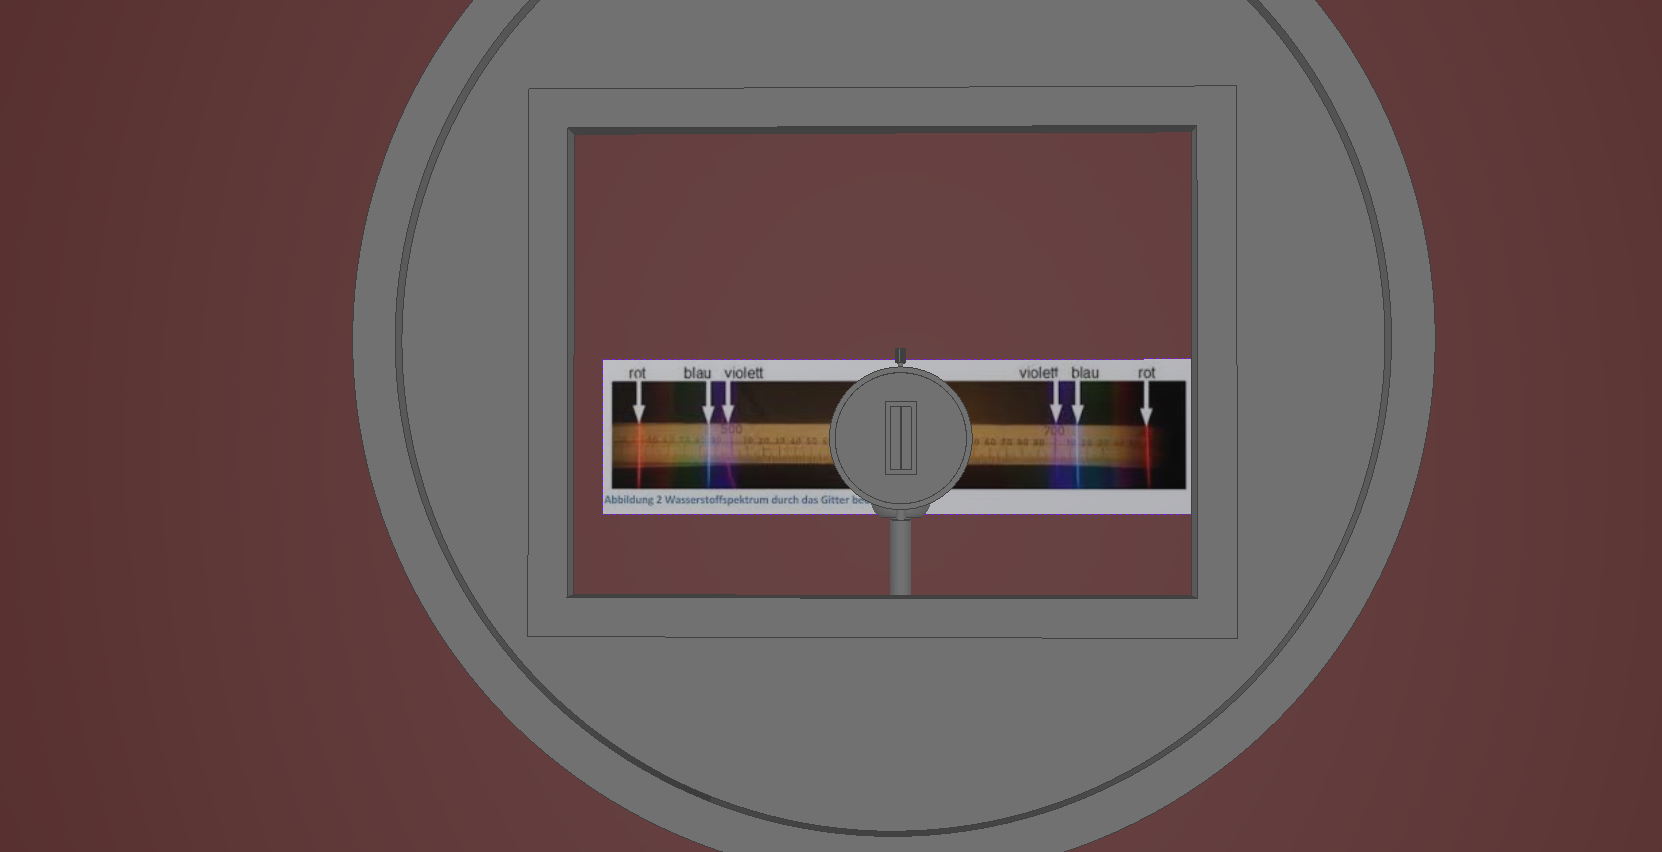
\includegraphics[width=\textwidth]{Gittersicht.png}
    \caption[Sicht durch das Gitter]{Sicht durch das Gitter}

    \vspace*{\floatsep}

    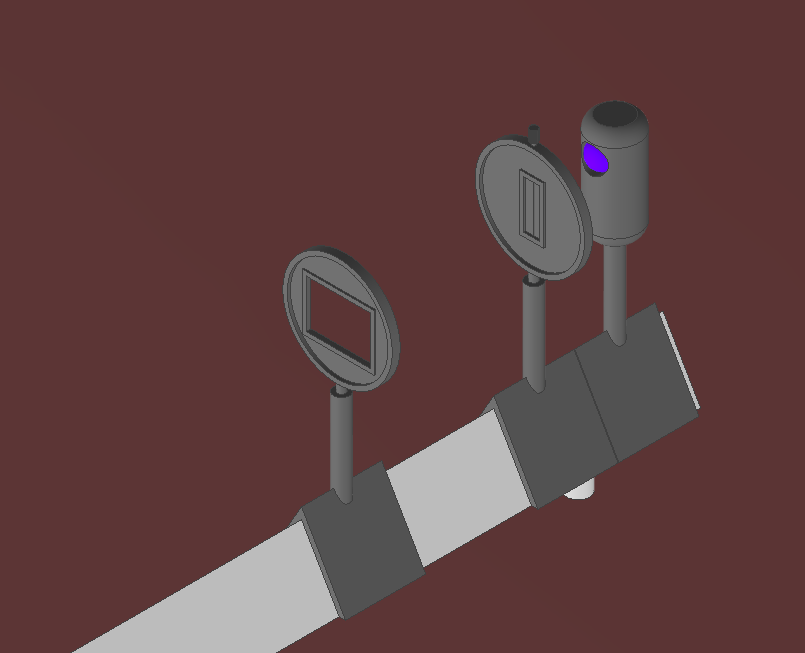
\includegraphics[width=\textwidth]{Perspektive.png}
    \caption[Perspektivische Ansicht]{Perspektivische Ansicht}
\end{figure}

\newpage

\subsection{Durchführung}
Nach dem Einschalten der Wasserstofflampe muss diese ein paar Sekunden aufwärmen.

Der Raum wird verdunkelt, das Diffraktionsgitter wird auf einen beliebigen Abstand vom Schirm ($l$) bewegt.
Bei der Betrachtung der virtuellen Abbildung durch das Gitter ist nun das Linienspektrum der Emission der Wasserstofflampe sichtbar.
Mit der Spaltgröße lässt sich die Schärfe der Linien einstellen.

Nun kann der Abstand zwischen den Maxima der einzelnen Wellenlängen über die 0. Ordnung abgelesen werden ($2*a$).
Der Maximaabstand $2a$ wird zusammen mit der Distanz zwischen Schirm und Gitter $l$ notiert.

Der Abstand $l$ kann nun beliebig oft verändert werden und die neuen Messwerte können notiert werden.

\newpage

\section{Auswertung}
\subsection{Messwerte}
\subsubsection{Abstände}
\begin{tabular}{ |c|c|c|c| }
    \hline
    $l/mm$ & $a_{rot}/mm$ & $a_{cyan}/mm$ & $a_{blau}/mm$ \\
    \hline
    \hline
    720 & 580 & 450 & 400 \\
    \hline
    700 & 580 & 445 & 400 \\
    \hline
    680 & 598 & 428 & 378 \\
    \hline
    660 & 580 & 412 & 370 \\
    \hline
    640 & 565 & 402 & 357 \\
    \hline
    600 & 490 & 350 & 310 \\
    \hline
    550 & 445 & 325 & 281 \\
    \hline
    500 & 400 & 288 & 255 \\
    \hline
    450 & 368 & 261 & 230 \\
    \hline
\end{tabular}

\subsubsection{Wellenlängen}
$\lambda = \sin(\arctan(\frac{x}{l})) * g$\\
$\lambda = \sin(\arctan(\frac{x}{l})) * \frac{1mm}{600}$\\\\
\textbf{Beispiel:} $l = 720mm$; $x = 580mm$ (rot)\\
$\lambda = \sin(\arctan(\frac{580mm}{720mm}))*\frac{1mm}{600}$\\
$\lambda = 622nm$\\

\begin{tabular}{ |c|c|c|c| }
    \hline
    $l/mm$ & $\lambda_{rot}/nm$ & $\lambda_{cyan}/nm$ & $\lambda_{blau}/nm$ \\
    \hline
    \hline
    720 & 622 & 497 & 446\\
    \hline
    700 & 637 & 504 & 457\\
    \hline
    680 & 670 & 500 & 446\\
    \hline
    660 & 670 & 496 & 449\\
    \hline
    640 & 673 & 499 & 447\\
    \hline
    600 & 630 & 466 & 416\\
    \hline
    550 & 625 & 463 & 412\\
    \hline
    500 & 618 & 461 & 411\\
    \hline
    450 & 630 & 464 & 412\\
    \hline
\end{tabular}

\newpage

\subsection{Visualisierung}
\subsubsection{Abstände}
\begin{tikzpicture}
    \begin{axis}[
        title={Messwerte},
        xlabel={l/mm},
        ylabel={a/mm},
        xmin=400, xmax=800,
        ymin=0, ymax=800,
        xtick={400, 500, 600, 700, 800},
        ytick={0, 100, 200, 300, 400, 500, 600, 700, 800},
        legend pos=south east,
        ymajorgrids=true,
        xmajorgrids=true,
        grid style=dashed,
    ]

    \addplot[
        color=red,
        mark=square,
    ]
    coordinates {
        (720,580)(700,580)(680,598)(660,580)(640,565)(600,490)(550,445)(500,400)(450,368)
    };

    \addplot[
        color=cyan,
        mark=square,
    ]
    coordinates {
        (720,450)(700,445)(680,428)(660,412)(640,402)(600,350)(550,318)(500,288)(450,261)
    };

    \addplot[
        color=blue,
        mark=square,
    ]
    coordinates {
        (720,400)(700,400)(680,378)(660,370)(640,357)(600,310)(550,281)(500,255)(450,230)
    };

    \addlegendentry{Messwerte (Rot)}
    \addlegendentry{Messwerte (Cyan)}
    \addlegendentry{Messwerte (Blau)}

    \end{axis}
\end{tikzpicture}

\subsubsection{Wellenlängen}
\begin{tikzpicture}
    \begin{axis}[
        title={Messwerte},
        xlabel={l/mm},
        ylabel={a/mm},
        xmin=400, xmax=800,
        ymin=0, ymax=800,
        xtick={400, 500, 600, 700, 800},
        ytick={0, 100, 200, 300, 400, 500, 600, 700, 800},
        legend pos=south east,
        ymajorgrids=true,
        xmajorgrids=true,
        grid style=dashed,
    ]

    \addplot[
        color=red,
        mark=square,
    ]
    coordinates {
        (720,622)(700,637)(680,670)(660,670)(640,673)(600,630)(550,625)(500,618)(450,630)
    };

    \addplot[
        color=cyan,
        mark=square,
    ]
    coordinates {
        (720,497)(700,504)(680,500)(660,496)(640,499)(600,466)(550,462)(500,461)(450,464)
    };

    \addplot[
        color=blue,
        mark=square,
    ]
    coordinates {
        (720,446)(700,457)(680,446)(660,449)(640,447)(600,416)(550,412)(500,411)(450,412)
    };

    \addlegendentry{Wellenlängen (Rot)}
    \addlegendentry{Wellenlängen (Cyan)}
    \addlegendentry{Wellenlängen (Blau)}

    \end{axis}
\end{tikzpicture}


\subsection{Statistik}

\subsubsection{Lineare Regression}
\large
$\sin(\arctan(\frac{x}{l})) = \frac{\lambda}{g} \Rightarrow x = \tan(\arcsin(\frac{\lambda}{g})) * l$ \\\\
$x(l) = \tan(\arcsin(\frac{\lambda}{g})) * l$ \\
$f(x) = m_s * x$\\\\
$m_s = \tan(\arcsin(m_s)) * g$\\
$\Rightarrow \lambda = \sin(\arctan(m_s)) * g$
\normalsize

\subsubsection{Daten}
\large
Mittelwert: $\overline{x} = \frac{\Sigma x_i}{N}$\\
Varianz (Stichprobenmessung): $\sigma^2 = \frac{\Sigma(x_i-\overline{x})^2}{N-1}$\\
Standardabweichung: $\sigma = \pm \sqrt{\sigma^2}$
\normalsize

\vspace{5mm}

\begin{tabular}{ |c|c|c|c| }
    \hline
    & rot & cyan & blau \\
    \hline
    \hline
    $\overline{\lambda}$ & $642nm$ & $484nm$ & $434nm$ \\
    \hline
    $\sigma$ & $23nm$ & $19nm$ & $19nm$ \\
    \hline
    \hline
    Literaturwert & $656nm$ & $486nm$ & $434nm$ \\
    \hline
    $\delta$ & $14nm$ & $2nm$ & $0nm$ \\
    \hline
    Abweichung & $2.1\%$ & $0.5\%$ & $0\%$ \\
    \hline
\end{tabular}

\newpage

\subsection{Fazit / Reflexion}
Die letzten Messwerte (die, dessen Abstand am geringsten ist) sind am genauesten,
da dort die Bilder, welche von uns mit einer Handykamera aufgenommen wurde,
am schärfsten waren.
Außerdem ist die Messreihe der roten Wellenlängen am ungenauesten,
da diese auf den Fotos die höchste Intensität hatte und damit
verschwommen dargestellt wurde und die Skala hierdurch verdeckt wurde.

Schlussendlich kommen wir auf eine Durschnittsabweichung von den Literaturwerten von $0.87\%$.
Hierbei ist zu beachten, dass die Abweichungen der Messreihe der cyanfarbenden
Wellenlängen nur eine Abweichung von $0.5\%$ darlegt und bei den Messwerten der
blauen Wellenlängen keine signifikante Abweichung besteht. Die blauen Messwerte
stellten stets eine sehr scharfe Linie dar.

\end{document}